\documentclass[9pt]{beamer}

% apparence
\usetheme{Singapore}
\usecolortheme{orchid}
\setbeamercolor{title}{
    use=structure,fg=white,bg=structure.fg!75!black
}
\useinnertheme[shadow]{rounded}

% numéro des slides
\addtobeamertemplate{navigation symbols}{}{
    \usebeamerfont{footline}
    \usebeamercolor[fg]{footline}
    \hspace{1em}
    \raisebox{2pt}{
        \insertframenumber/\inserttotalframenumber
    }
}

% réduire l'espace sous les titres de slides
\addtobeamertemplate{frametitle}{}{\vspace*{-5mm}}

\makeatletter

% afficher/masquer dans miniframes
\let\beamer@writeslidentry@miniframeson=\beamer@writeslidentry
\def\beamer@writeslidentry@miniframesoff{
    \expandafter\beamer@ifempty\expandafter{\beamer@framestartpage}{}
    {\clearpage\beamer@notesactions}
}

\newcommand*{\miniframeson}{
    \let\beamer@writeslidentry=\beamer@writeslidentry@miniframeson
}

\newcommand*{\miniframesoff}{
    \let\beamer@writeslidentry=\beamer@writeslidentry@miniframesoff
}

% séparation épaisse dans un tableau
\def\hlinewd#1{
\noalign{\ifnum0=`}\fi\hrule \@height #1
\futurelet\reserved@a\@xhline}

\makeatother

% packages
\usepackage{setspace}
\usepackage{graphicx}
\usepackage{algorithm, algpseudocode}
\usepackage[dvipsnames]{xcolor}

% titre du beamer
\title{Learning Observation Model for SLAM via Random Fourier Features in a Kernel Kalman Filter}

\author{
    Bastien HUBERT\inst{1, 2},
    Karim DAHIA\inst{1},\\
    Nicolas MERLINGE\inst{1},
    Audrey GIREMUS\inst{2}
}

\institute{
    \inst{1} ONERA, DTIS, IGNC\quad
    \inst{2} Université de Bordeaux, CNRS, IMS
}

\date{}

\titlegraphic{
    \vspace{-\baselineskip}
    
\includegraphics[width=10cm]{../../Images/Logo ONERA IMS.pdf}
}

% début du beamer
\begin{document}

\begin{frame}

\begin{center}
    \includegraphics[width=2cm]{../../Images/Logo FUSION 2026.png}
    \hspace{1cm}
    \raisebox{5pt}{\includegraphics[width=2cm]{../../Images/Logo IEEE.png}}
    \vspace{-\baselineskip}
\end{center}

\titlepage

\end{frame}

\logo{
    \includegraphics[width=1cm]{../../Images/Logo FUSION 2026.png}
    \hspace{2mm}
    \raisebox{1pt}{\includegraphics[width=1cm]{../../Images/Logo IEEE.png}}
    \hspace{4.7cm}
    
\includegraphics[width=5cm]{../../Images/Logo ONERA IMS.pdf}
}

\section{Introduction}

\begin{frame}{Context: simultaneous localisation and mapping}

\begin{block}{Autonomous navigation}
    \begin{itemize}
    \item Estimating an agent's state while exploring an unknown environment
    \item Inertial navigation drifts $\rightarrow$ fusion with an exteroceptive sensor
    \item[$\Rightarrow$]Field-based navigation: comparison of measurements with a map
    \end{itemize}
\end{block}

\begin{block}{Simultaneous Localisation and Mapping (SLAM)}
    \begin{itemize}
    \item No map available beforehand
    \item[$\Rightarrow$]Concurrently build the map and estimate the state relative to it
    \item Landmark-based SLAMs: geometric features observable at a distance
    \item Field-based SLAMs: local measurements of an unknown spatial field
    \end{itemize}
\end{block}

\end{frame}

\begin{frame}{Field-based SLAM with an unknown observation model}

\begin{block}{Problem}
    \begin{itemize}
    \item Classical filtering assumes a known observation function $h_k$
    \item $h_k$ is a complex, poorly-parameterised, unknown physical field
    \item Data-driven solutions (NN, GP) $\rightarrow$ break recursivity and store past data
    \end{itemize}
\end{block}

\begin{block}{Proposed approach}
    \begin{itemize}
    \item Navigation in a RKHS $\rightarrow$ handles non-linearities without linearisation
    \item Filtering: Adaptive Kernel Kalman Filter (AKKF)
    \item Learning $h_k$ online with Random Fourier Features (RFF) and Recursive Least Squares (RLS)
    \item[$\Rightarrow$]Recursive SLAM with no analytical model and fixed per-step cost
    \end{itemize}
\end{block}

\end{frame}

\section{Bayesian filtering in a RKHS}

\begin{frame}{Bayesian estimation}

\begin{block}{Discrete state-space model (DSSM)}
    \begin{itemize}
    \item\hfill$\left\{\begin{aligned}
    x_k&=f_k(x_{k-1},\nu_k)&&\text{recursive dynamical process}\\
    z_k&=h_k(x_k)+\eta_k&&\text{measurement equation}
    \end{aligned}\right.$\hfill(1)
    \end{itemize}
\end{block}

\begin{block}{Optimal Bayesian filter}
    \begin{itemize}
    \item Goal: recursively estimate the PDF $p(x_k|z_{1:k})$
    \item Prediction with the Chapman-Kolmogorov equation:\\
    \hfill$\displaystyle p(x_k|z_{1:k-1})=\underbrace{\int p(x_k|x_{k-1})\:p(x_{k-1}|z_{1:k-1})\:dx_{k-1}}_{\text{no analytical solution in general}}$\hfill(2)
    \item Correction with Bayes' formula:\\
    \hfill$\displaystyle p(x_k|z_{1:k})\propto p(z_k|x_k)\:p(x_k|z_{1:k-1})$\hfill(3)
    \end{itemize}
\end{block}

\end{frame}

\begin{frame}{Bayesian estimation}

\begin{columns}[onlytextwidth]
\begin{column}{0.6\textwidth}

\begin{block}{Kalman filter}
    \begin{itemize}
    \item Optimal in the linear Gaussian case
    \item Linearisation errors for strongly non-linear/non-injective models
    \end{itemize}
\end{block}

\begin{block}{Particle filter}
    \begin{itemize}
    \item Monte-Carlo approximation of the PDFs
    \item Robust, but high computational cost
    \item Sample degeneracy in high dimension
    \end{itemize}
\end{block}

\end{column}
\begin{column}{0.35\textwidth}

\begin{center}
    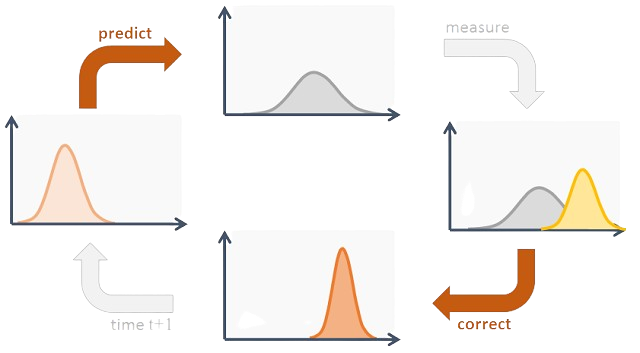
\includegraphics[width=\textwidth]{../../Images/Étapes du filtre de Kalman avec images.png}
\end{center}

\end{column}
\end{columns}

\begin{block}{Kernel-based methods}
    \begin{itemize}
    \item Cast (1) into a RKHS $\rightarrow$ distributions become linear
    \item[$\Rightarrow$]Weighted ensemble Kalman-like recursion with no explicit linearisation
    \end{itemize}
\end{block}

\end{frame}

\begin{frame}{RKHS and kernel mean embedding}

\begin{block}{Reproducing Kernel Hilbert Space $(\mathcal{H},\langle\cdot|\cdot\rangle_{\mathcal{H}},k)$}
    \begin{itemize}
    \item Reproducing property:\\
    \hfill$\displaystyle\forall f\in\mathcal{H},\forall x\in\Omega,\:\langle f|k(x,\cdot)\rangle_{\mathcal{H}}=f(x)$\hfill(4)
    \end{itemize}
\end{block}

\begin{block}{Kernel mean embedding (KME)}
    \begin{itemize}
    \item Expectations become linear evaluations in $\mathcal{H}$:\\
    \hfill$\displaystyle\mathbb{E}_X(f(X))=\langle f|\mu_X\rangle_{\mathcal{H}},\qquad\mu_X\triangleq\mathbb{E}_X(k(X,\cdot))\approx\frac{1}{N}\sum_{i=1}^Nk(x^i,\cdot)$\hfill(5)
    \item Conditioning is also linear:\\
    \hfill$\begin{gathered}
    \mu_{X|z}=\mathcal{C}_{XZ}\:(\mathcal{C}_{ZZ}+\lambda_{\mathcal{H}}I)^{-1}\:k(z,\cdot)\\
    \mathcal{C}_{XZ}\triangleq\mathbb{E}(k(X,\cdot)\otimes k(Z,\cdot))\approx\frac{1}{N}\sum_{i=1}^Nk(x^i,\cdot)k(z^i,\cdot)^\top
    \end{gathered}$\hfill(6)
    \item Empirical estimator:\\
    \hfill$\displaystyle\mathbb{E}_{X|z}(X)\approx\hat{x}=\sum_{i=1}^{N}w^ix^i,\qquad\mathbf{w}\triangleq(k(\mathbf{z},\mathbf{z})+\lambda_{\mathcal{H}}I)^{-1}k(\mathbf{z},z)$\hfill(7)
    \end{itemize}
\end{block}

\end{frame}

\begin{frame}{The Adaptive Kernel Kalman Filter (AKKF)}

\begin{block}{Principle}
    \begin{itemize}
    \item State-space model embedded in two RKHS $\mathcal{H}_x$, $\mathcal{H}_z$
    \item Kalman optimality preserved in the feature space
    \item Weights are propagated through a prediction/correction/resampling loop
    \end{itemize}
\end{block}

\begin{block}{One AKKF iteration}
\begin{algorithmic}\setstretch{1.35}
    \State$\forall i,\:x_k^i\sim p(x_k|\tilde{x}_{k-1}^i)$\Comment{DSSM prediction}
    \State$P_{k|k-1}\gets\tilde{P}_{k-1|k-1}+\frac{1}{N}D_kD_k^\top$\Comment{RKHS prediction}
    \State$\forall i,\:z_k^i\sim p(z_k|x_k^i)$\Comment{\textcolor{BrickRed}{DSSM correction: requires $h_k$}}
    \State$\mathbf{w}_k\gets\tilde{\mathbf{w}}_{k-1}+Q_k(k_z(\mathbf{z}_k,z_k)-k_z(\mathbf{z}_k,\mathbf{z}_k)\tilde{\mathbf{w}}_{k-1})$\Comment{RKHS correction}
    \State$P_{k|k}\gets P_{k|k-1}-Q_kk_z(\mathbf{z}_k,\mathbf{z}_k)P_{k|k-1}$
    \State$\forall i,\:\tilde{x}_k^i\sim\mathcal{N}(\hat{x}_k, \hat{P}_k)$\Comment{DSSM resampling}
    \State$\tilde{\mathbf{w}}_k\gets T_k\mathbf{w}_k,\qquad\tilde{P}_{k|k}\gets T_kP_{k|k}T_k^\top$\Comment{RKHS resampling}
\end{algorithmic}
\end{block}

\end{frame}

\section{Learning the observation model}

\begin{frame}{Learning an unknown observation model}

\begin{block}{Modelling the observation function}
    \begin{itemize}
    \item Evaluation of the unknown $h_k$ needed for the AKKF correction step
    \item Moore-Aronszajn theorem:\\
    \hfill$\mathcal{H}_x=\overline{\text{span}}\{k_x(x,\cdot),\:x\in\Omega_x\}$\hfill(8)
    \item Approximation of $h_k\in\mathcal{H}_x$:\\
    \hfill$\displaystyle h_k(x)\approx\sum_{i=1}^{N}\tilde{a}^i\:k_x(x_k^i,x)$\hfill(9)
    \item But evaluation within $(\mathcal{H}_x,\langle\cdot|\cdot\rangle_{\mathcal{H}_x},k_x)$ is non-trivial
    \item[$\Rightarrow$]Need an explicit finite-dimensional approximation of $k_x$
    \end{itemize}
\end{block}

\end{frame}

\begin{frame}{Random Fourier Features (RFF)}

\begin{block}{Bochner's theorem}
    \begin{itemize}
    \item Assuming that $k_x$ is stationary:\\
    \hfill$\displaystyle k_x(x-x')=\int\exp\left(j\omega^\top(x-x')\right)\:p(d\omega)=\mathbb{E}_\omega\left(\varphi_\omega(x)^\top\varphi_\omega(x')\right)$\hfill(10)
    \item$k_x$ is the Fourier transform of a spectral density $p(\omega)$
    \end{itemize}
\end{block}

\begin{block}{Finite-dimensional approximation}
    \begin{itemize}
    \item Fourier features:\\
    \hfill$\displaystyle\varphi:x\mapsto\sqrt{\tfrac{2}{D}}\:\left[\cos(\omega_1^\top x + b_1),\cdots,\cos(\omega_D^\top x + b_D)\right]^\top$\hfill(11)\vspace{2mm}\\
    where $\omega_d\sim p(\omega)$ and $b_d\sim \mathcal{U}([0, 2\pi])$, $d\in[\![1,D]\!]$
    \item Kernel approximation:\\
    \hfill$k(x,x')\approx\varphi(x)^\top\varphi(x')$\hfill(12)
    \item[$\Rightarrow$]Approximation of $h_k$ using (9):\\
    \hfill$\displaystyle h_k(x)\approx\mathbf{a}^\top\varphi(x),\qquad\mathbf{a}\in\mathbb{R}^D$\hfill(13)
    \end{itemize}
\end{block}

\end{frame}

\begin{frame}{Recursive Least Squares (RLS)}

\begin{block}{Learning the observation weights $a$}
    \begin{itemize}
    \item Objective: minimising the loss:\\
    \hfill$\displaystyle J:\mathbf{a}\mapsto\sum_{l=1}^k\beta^{k-l}\:\left\|z_l-\mathbf{a}^\top\varphi(\hat{x}_l)\right\|^2+\beta^k\lambda_{RLS}\|\mathbf{a}\|^2$\hfill(14)
    \item Training pairs: AKKF estimate $\hat{x}_k$ and observation $z_k$
    \item[$\Rightarrow$]Recursive algorithm: fixed cost and no stored history
    \end{itemize}
\end{block}

\begin{block}{One RLS iteration}
\begin{algorithmic}\setstretch{1.35}
    \State$\mathbf{k}_k\gets R_{k-1}\varphi(\hat{x}_k)\left(\beta+\varphi(\hat{x}_k)^\top R_{k-1}\varphi(\hat{x}_k)\right)^{-1}$ \Comment{Kalman-like gain}
    \State$\mathbf{a}_k\gets\mathbf{a}_{k-1}+\mathbf{k}_k\left(z_k-\mathbf{a}_{k-1}^\top\varphi(\hat{x}_k)\right)$\Comment{Weight update}
    \State$R_k\gets\frac{1}{\beta}\left(I-\mathbf{k}_k\varphi(\hat{x}_k)^\top\right)R_{k-1}$\Comment{Covariance update}
\end{algorithmic}
\end{block}

\end{frame}

\begin{frame}{RFF/RLS AKKF SLAM}

\begin{block}{Joint state estimation and map learning}
    \begin{itemize}
    \item Prediction: standard AKKF propagation through the state transition model
    \item Correction: observation simulation from the current learned model, then kernel filtering
    \item Map update: RLS update of the observation model
    \item Resampling: keep particles and RKHS approximations consistent
    \end{itemize}
\end{block}

\begin{block}{Algorithm overview}
\begin{algorithmic}\setstretch{1.35}
    \State$\forall i,\:x_k^i\sim p(x_k|\tilde{x}_{k-1}^i)$\Comment{DSSM+RKHS prediction}
    \State \textcolor{BrickRed}{$\forall i,\:z_k^i=\mathbf{a}_{k-1}^\top\varphi(x_k^i)+\eta_k^i$}\Comment{\textcolor{BrickRed}{DSSM/RFF correction}}
    \State$\mathbf{w}_k\gets\tilde{\mathbf{w}}_{k-1}+Q_k(k_z(\mathbf{z}_k,z_k)-k_z(\mathbf{z}_k,\mathbf{z}_k)\tilde{\mathbf{w}}_{k-1})$\Comment{RKHS correction}
    \State \textcolor{BrickRed}{$\mathbf{a}_k\gets\mathbf{a}_{k-1}+\mathbf{k}_k(z_k-\mathbf{a}_{k-1}^\top\varphi(\hat{x}_k))$}\Comment{\textcolor{BrickRed}{RFF/RLS map update}}
    \State$\forall i,\:\tilde{x}_k^i\sim\mathcal{N}(\hat{x}_k, \hat{P}_k)$\Comment{DSSM+RKHS resampling}
\end{algorithmic}
\end{block}

\end{frame}

\section{Numerical results}

\begin{frame}{Simulation scenario}

\begin{columns}[onlytextwidth]
\begin{column}{0.58\textwidth}

\begin{block}{Setup}
    \begin{itemize}
    \item Spiral trajectory over $100$ time steps
    \item Non-injective, non-linear observation field
    \item $100$ Monte-Carlo runs, $1000$ particles
    \end{itemize}
\end{block}

\end{column}
\begin{column}{0.39\textwidth}

\begin{center}
    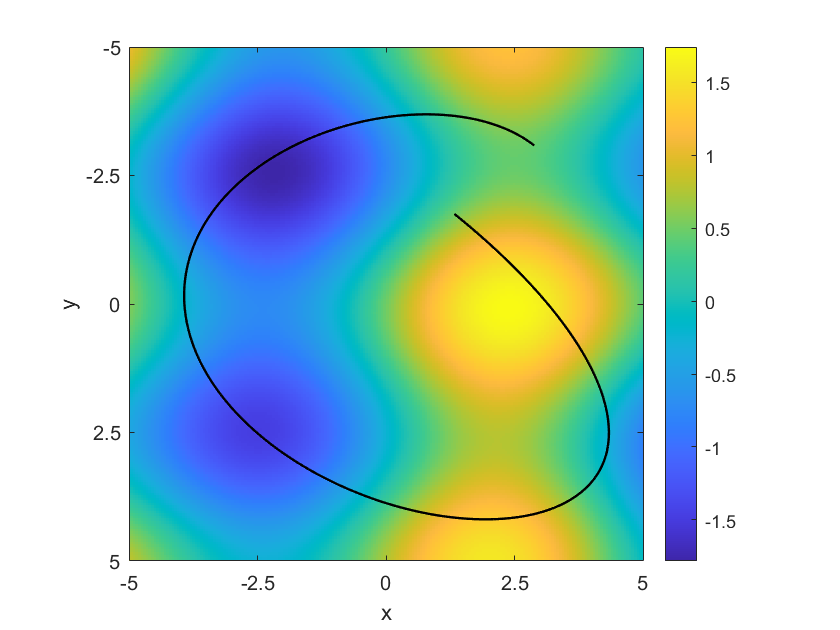
\includegraphics[width=\textwidth]{../../Images/Trajectoire FUSION 2026.png}
\end{center}

\end{column}
\end{columns}

\begin{block}{Compared filters}
    \begin{itemize}
    \item 3 PFs with a known degraded model\\
    \hfill$h_\alpha=(1+\varepsilon)h,\qquad\varepsilon\sim\mathcal{N}(0,\alpha),\qquad\alpha\in\{0,0.1,0.5\}$\hfill(15)
    \item Proposed SLAM ($D = 500$)
    \end{itemize}
\end{block}

\end{frame}

\begin{frame}{State estimation performance}

\begin{center}
    \includegraphics[height=5cm]{../../Images/RMSE Trajectoire FUSION 2026.png}
\end{center}

\begin{block}{Analysis}
    \begin{itemize}
    \item SLAM must learn $h_k$ $\rightarrow$ higher early error than any PF
    \item Asymptotic error equal to the most degraded PF without prior model
    \item Transient-to-asymptotic decrease similar to the PF with the perfect model
    \end{itemize}
\end{block}

\end{frame}
\begin{frame}{Observation model reconstruction}

\begin{columns}[onlytextwidth]
\begin{column}{0.5\textwidth}

\begin{center}
    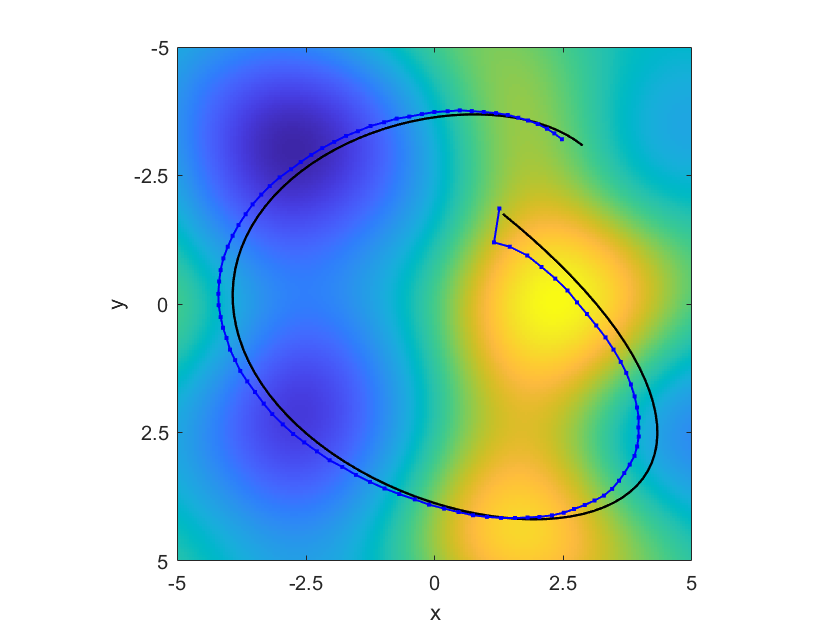
\includegraphics[width=\textwidth]{../../Images/Carte reconstruite FUSION 2026.png}
\end{center}

\end{column}
\begin{column}{0.5\textwidth}

\begin{center}
    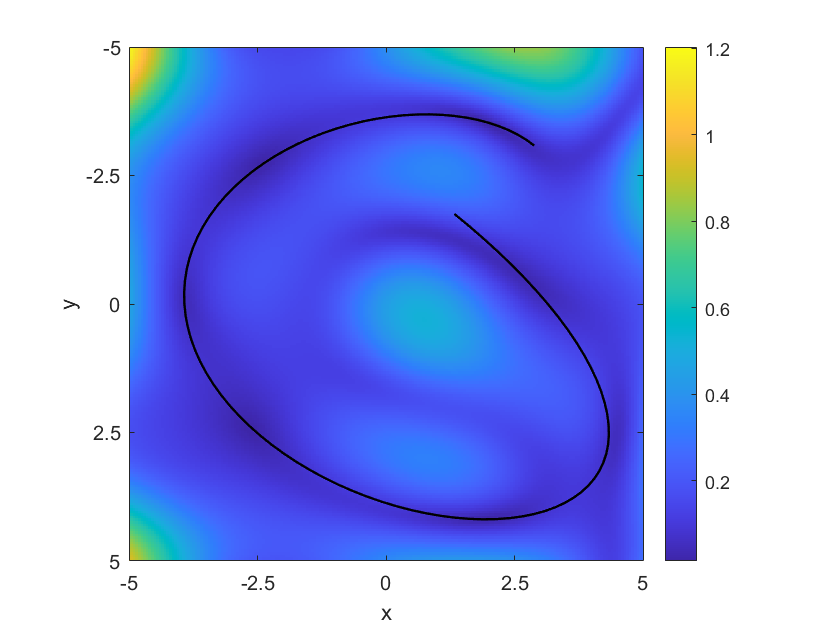
\includegraphics[width=\textwidth]{../../Images/RMSE carte FUSION 2026.png}
\end{center}

\end{column}
\end{columns}

\begin{block}{Map quality}
    \begin{itemize}
    \item Mean error $0.21$, reduced to $0.07$ along the trajectory
    \item Outer peaks: extrapolation errors away from the explored path
    \item Inner peaks: localisation bias propagated into the map through $\hat{x}_k$
    \end{itemize}
\end{block}

\end{frame}

\section{Conclusion}

\begin{frame}{Conclusion and future work}

\begin{block}{Our work}
    \begin{itemize}
    \item A fully recursive SLAM framework combining AKKF + RFF + RLS
    \item Joint state estimation and online observation model learning in a RKHS
    \item Extends Bayesian filtering to highly non-linear, non-injective systems with no analytical observation model or prior data samples
    \item Performance comparable to PFs with a known degraded model
    \end{itemize}
\end{block}

\begin{block}{Perspectives}
    \begin{itemize}
    \item Explicitly integrate state uncertainty into the map regression
    \item Joint estimation of observation parameters with the state
    \item Validation on real-world field-based navigation applications
    \end{itemize}
\end{block}

\end{frame}

\end{document}
